%%%%%%%%%%%%%%%%%%%%%%%%%%%%%%%%%%%%%%%%%
% Beamer Presentation
% LaTeX Template
% Version 1.0 (10/11/12)
%
% This template has been downloaded from:
% http://www.LaTeXTemplates.com
%
% License:
% CC BY-NC-SA 3.0 (http://creativecommons.org/licenses/by-nc-sa/3.0/)
%
%%%%%%%%%%%%%%%%%%%%%%%%%%%%%%%%%%%%%%%%%

%----------------------------------------------------------------------------------------
%	PACKAGES AND THEMES
%----------------------------------------------------------------------------------------

\documentclass{beamer}

\mode<presentation> {

% The Beamer class comes with a number of default slide themes
% which change the colors and layouts of slides. Below this is a list
% of all the themes, uncomment each in turn to see what they look like.

%\usetheme{default}
%\usetheme{AnnArbor}
%\usetheme{Antibes}
%\usetheme{Bergen}
%\usetheme{Berkeley}
%\usetheme{Berlin}
%\usetheme{Boadilla}
%\usetheme{CambridgeUS}
%\usetheme{Copenhagen}
%\usetheme{Darmstadt}
%\usetheme{Dresden}
%\usetheme{Frankfurt}
%\usetheme{Goettingen}
%\usetheme{Hannover}
%\usetheme{Ilmenau}
%\usetheme{JuanLesPins}
%\usetheme{Luebeck}
\usetheme{Madrid}
%\usetheme{Malmoe}
%\usetheme{Marburg}
%\usetheme{Montpellier}
%\usetheme{PaloAlto}
%\usetheme{Pittsburgh}
%\usetheme{Rochester}
%\usetheme{Singapore}
%\usetheme{Szeged}
%\usetheme{Warsaw}

% As well as themes, the Beamer class has a number of color themes
% for any slide theme. Uncomment each of these in turn to see how it
% changes the colors of your current slide theme.

%\usecolortheme{albatross}
%\usecolortheme{beaver}
%\usecolortheme{beetle}
%\usecolortheme{crane}
%\usecolortheme{dolphin}
%\usecolortheme{dove}
%\usecolortheme{fly}
%\usecolortheme{lily}
%\usecolortheme{orchid}
%\usecolortheme{rose}
%\usecolortheme{seagull}
%\usecolortheme{seahorse}
%\usecolortheme{whale}
%\usecolortheme{wolverine}

%\setbeamertemplate{footline} % To remove the footer line in all slides uncomment this line
%\setbeamertemplate{footline}[page number] % To replace the footer line in all slides with a simple slide count uncomment this line

%\setbeamertemplate{navigation symbols}{} % To remove the navigation symbols from the bottom of all slides uncomment this line
}

\usepackage{bm} % bold in math
\usepackage{graphicx} % Allows including images
\usepackage{booktabs} % Allows the use of \toprule, \midrule and \bottomrule in tables

\newcommand{\ifnf}{\Leftrightarrow}
\newcommand{\bra}[1]{\left(#1\right)}
\newcommand{\cbra}[1]{\left\{#1\right\}}
\newcommand{\sbra}[1]{\left[#1\right]}
\newcommand{\e}[1]{$\displaystyle{#1}$}
\newcommand{\al}[1]{\begin{align*}#1\end{align*}}
\newcommand{\defeq}{\overset{\mathrm{def}}{=}}
\newcommand{\abs}[1]{\left\lvert#1\right\rvert}
\newcommand{\norm}[1]{\left\lVert#1\right\rVert}
\newcommand{\inner}[2]{\left\langle #1, #2 \right\rangle}
\newcommand{\floor}[1]{\left\lfloor#1\right\rfloor}
\newcommand{\ceil}[1]{\left\lceil#1\right\rceil}
\newcommand{\mres}{\mathbin{\vrule height 1.6ex depth 0pt width
0.13ex\vrule height 0.13ex depth 0pt width 1.3ex}}


%----------------------------------------------------------------------------------------
%	TITLE PAGE
%----------------------------------------------------------------------------------------

\title[MAS583 Final Presentation]{A Propensity-Score-Adjustment Method\\ for Nonignorable Nonresponse} % The short title appears at the bottom of every slide, the full title is only on the title page

\author{Junho Han} % Your name
\institute[MathSci, KAIST] % Your institution as it will appear on the bottom of every slide, may be shorthand to save space
{
MathSci, KAIST \\ % Your institution for the title page
%\medskip
%MAS583, Statistical Analysis with Incomplete Data (Prof. Jae Kwang Kim)
}
\date{\today} % Date, can be changed to a custom date

\begin{document}

\begin{frame}
\titlepage % Print the title page as the first slide
\end{frame}

\begin{frame}
\frametitle{Table of Contents} % Table of contents slide, comment this block out to remove it
\tableofcontents % Throughout your presentation, if you choose to use \section{} and \subsection{} commands, these will automatically be printed on this slide as an overview of your presentation
\end{frame}

%----------------------------------------------------------------------------------------
%	PRESENTATION SLIDES
%----------------------------------------------------------------------------------------

%------------------------------------------------
\section{Introduction and Basic Setup} % Sections can be created in order to organize your presentation into discrete blocks, all sections and subsections are automatically printed in the table of contents as an overview of the talk
%------------------------------------------------

%------------------------------------------------
%=========================
\subsection{Propensity Score Method for Nonresponse}
%=========================
\begin{frame}
\frametitle{Propensity Score Method for Nonresponse}
Nonresponse has become a major problem in sample surveys as participation rates have declined in many surveys. Weighting adjustments are commonly used to adjust for unit nonresponse. \\~\\

Classical approaches include poststratification (Holt and Smith 1979), regression weighting (Bethlehem 1988), and raking ratio estimation (Deville, Särndal, and Sautory 1993). \textbf{Propensity-score weighting}, which increases the sampling weights of the respondents using their inverse response probabilities, is a popular approach for handling unit nonresponse.

\al{U_{ps}\bra{\theta}=\sum_{i=1}^{n} \delta_{i} {\pi_{i}^{-1}U_i\bra{\theta}} = 0.}
\end{frame}

\begin{frame}
\frametitle{Propensity Score Method for Nonresponse}
\underline{Setup}
\begin{itemize}
\item \e{x_i}s are always observed and \e{y_i} is observed iff \e{\delta_i=1}.
\item The response mechanism is \e{\pi_i\bra{\phi; x_i, y_i} = pr\bra{\delta_i=1 | x_i, y_i}}.
\end{itemize}\bigskip

\underline{Ignorable Nonresponse} (missing at random)
\al{\sum_{i=1}^{n} \delta_{i} {\pi_{i}^{-1}\bra{\hat\phi; x_i}U_i\bra{\theta; x_i, y_i}} = 0.}\\~\\

\underline{Nonignorable Nonresponse}
\al{\sum_{i=1}^{n} \delta_{i} {\pi_{i}^{-1}\bra{\hat\phi; x_i, \bm{y_i}}U_i\bra{\theta; x_i, y_i}} = 0.}
\end{frame}

%=========================
\subsection{Existing Methods}
%=========================
\begin{frame}
\frametitle{Existing Methods}
\underline{Generalized Method of Moments}\\\medskip
Get \e{\hat\phi_{ck}} from the following calibration condition:
\al{\sum_{i=1}^{n} \cbra{\delta_{i} \pi_{i}^{-1}\bra{\phi; x_i, y_i} - 1}\bra{1, x_i} = 0.}
This method is efficient since it doesn't assmue any outcome models, i.e. \e{f\bra{y|x;\beta}}.
It is first proposed by \textit{Chang and Kott(2008)}.
\end{frame}

\begin{frame}
\frametitle{Existing Methods}
\underline{Fully Parametric}\\\medskip
Get \e{\phi_{mle}} from the mean score function (normal approach):
\al{\bar{\bm{S}}\bra{\phi}=\sum_{i=1}^{n} \sbra{
	\delta_{i}\bm{s_i}\bra{\phi; y_i} + \bra{1-\delta_i}E\cbra{\bm{s_i}\bra{\phi; Y}|x_i, \delta_{i}=0}}.}
To solve it, we need \e{f\bra{y|x, \delta=0}}. Fully parametric approach specifies \e{f\bra{y|x; \beta}} parametrized by \e{\beta} to derive \al{f\bra{y|x, \delta=0} = f\bra{y|x} \frac{pr\bra{\delta=0|x, y}}{E\cbra{pr\bra{\delta=0|x, Y}| x}}.}
However, this can be very sensitive to failure of the assumed model because it assumes the whole model over unobserved data.
\end{frame}

%------------------------------------------------
\section{Proposed Method}
%------------------------------------------------

\begin{frame}
\frametitle{Proposed Method}
\underline{Summary}
\begin{itemize}
\item It assumes only \e{f\bra{y|x, \delta=1; \gamma}} which is relatively easy to verify from the observed part of samples rather than \e{f\bra{y|x; \beta}}. So it is more robust than the fully parametric approach for an incorrectly specified outcome model.
\item It is more efficient than both GMM and FP in terms of accuracy or variance of estimates.
\item It suggests a novel computational tool applied to the empirical distribution of the response mechanism.
\end{itemize}\bigskip
\end{frame}

\begin{frame}
\frametitle{Proposed Method}
Let \e{f_i(y|x) = f(y|x,\delta=i)} and \e{E_i\cbra{\cdot} = E\cbra{\cdot|\delta=i}}.
The outcome model under nonresponse can be represented as
\al{f_0(y|x) = f_1(y|x) \frac{\bm{O}(x, y)}{E_1\cbra{\bm{O}(x, Y)|x}}}\smallskip where
\e{\bm{O}(x, y) = pr(\delta=0|x,y; \phi)/pr(\delta=1|x,y; \phi)}.
Using this formula, the mean score function can be computed by\smallskip
\al{\bar{\bm{S}}\bra{\phi}=\sum_{i=1}^{n} \sbra{
	\delta_{i}\bm{s_i}\bra{\phi; y_i} +
	\bra{1-\delta_i}\frac{E_1\cbra{\bm{s_i}\bra{\phi; Y}\bm{O}\bra{x, Y}|x_i}}
					   {E_1\cbra{\bm{O}\bra{x, Y}|x_i}}}.}
\end{frame}

\begin{frame}
\frametitle{Proposed Method}
Before getting \e{\hat\phi_{p}} from \e{\bar{\bm{S}}\bra{\phi}=0}, we need to compute a consistent estimator \e{\hat\gamma} for \e{f_1(y|x)=f_1(y|x;\gamma)}. Indeed, \e{\bar{\bm{S}}\bra{\phi}=\bar{\bm{S}}\bra{\phi, \gamma}}.\\~\\

Since \e{\gamma} only involves the observed part of samples, \e{\hat\gamma} is a solution of\smallskip
\al{\bm{S}\bra{\gamma} = \sum_{i=1}^{n} \delta_i \bm{s_i}\bra{\gamma}
					= \sum_{i=1}^{n} \delta_i \frac{\partial \log f_1\bra{y_i|x_i;\gamma}}{\partial \gamma} = 0.}\smallskip

This is a relatively easy step compared to the main part if \e{f_1} is appropriately specified. After finding \e{\hat\gamma}, we let \e{\bar{\bm{S}}\bra{\phi}=\bar{\bm{S}}\bra{\phi, \hat\gamma}}.
\end{frame}


\begin{frame}
\frametitle{Proposed Method}
\al{\bar{\bm{S}}\bra{\phi}=\sum_{i=1}^{n} \sbra{
	\delta_{i}\bm{s_i}\bra{\phi; y_i} +
	\bra{1-\delta_i}\frac{E_1\cbra{\bm{s_i}\bra{\phi; Y}\bm{O}\bra{x, Y}|x_i}}
					   {E_1\cbra{\bm{O}\bra{x, Y}|x_i}}}.}\smallskip

However, the expectation part is computationally challenging; so we use 2-steps of imporance sampling technique to resolve it.\\~\\

Let \e{\bm{Q}(x, y) = \bm{s_i}\bra{\phi; Y}\bm{O}\bra{x, Y}} or \e{\bm{O}\bra{x, Y}}, and we approximate each of \e{E_1\cbra{\bm{Q}(x, Y)|x_i}}.
\end{frame}

\begin{frame}
\frametitle{Proposed Method}
\underline{Step 1}
\al{E_1\cbra{\bm{Q}(x, Y)|x_i} \approx n_{r}^{-1}\sum_{\delta_j=1} \bm{Q}\bra{x_i, y_j} \frac{f_1\bra{y_j|x_i}}{f_1\bra{y_j}}}\\

\underline{Step 2}
\al{f_1\bra{y_j} = \int f_1\bra{y_j|x} f_1\bra{x} dx \approx n_{r}^{-1} \sum_{\delta_k=1}f_1\bra{y_j|x_k}}\\~\\

Applying this two importance sampling approximations to the original equation, we earn new approximate mean score function \e{\bar{\bm{S_2}}\bra{\phi}}. Moreover, we could estimate \e{\phi} by EM algorithm.
\end{frame}

\begin{frame}
\frametitle{Proposed Method}
\underline{Algorithm}
\begin{enumerate}
\item Get \e{\hat\gamma} from \e{
	\bm{S}\bra{\gamma} = \sum_{i=1}^{n} \delta_i \frac{\partial \log f_1\bra{y_i|x_i;\gamma}}{\partial \gamma} = 0.}
\item With \e{\bar{\bm{S_2}}\bra{\phi} = \bar{\bm{S_2}}\bra{\phi, \hat\gamma}}, obtain \e{\hat\phi_p} by EM algorithm:
		\al{\hat\phi^{(t+1)} \leftarrow \text{ solve } \bar{\bm{S_2}}\bra{\phi \middle| \hat\phi^{(t)}} = 0.}
\item Get \e{\hat\theta_p} by propensity-score method:
		\al{U_{ps}\bra{\theta}=\sum_{i=1}^{n} \delta_{i} {\pi_{i}^{-1}\bra{\hat\phi_p}U_i\bra{\theta}} = 0.}
\end{enumerate}\bigskip
\end{frame}
%------------------------------------------------
\section{Asymptotic Properties}
%------------------------------------------------

\begin{frame}
\frametitle{Asymptotic Properties}
\begin{block}{Theorem 1 (Asymptotic Normality)}
\al{\sqrt{n}\bra{\hat\phi_p - \phi_0} &\rightarrow N\bra{0, \Sigma_\phi}\\
	\sqrt{n}\bra{\hat\theta_p - \theta_0} &\rightarrow N\bra{0, \sigma^2_\theta}}
\vspace{2mm}
\end{block}
\end{frame}

\begin{frame}
\frametitle{Asymptotic Properties}
\begin{figure}
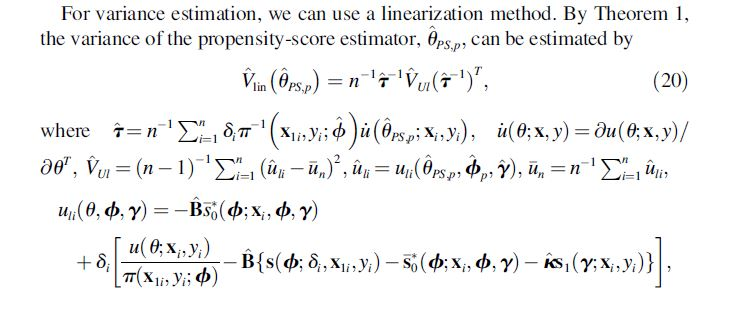
\includegraphics[width=1\linewidth]{linvar.jpg}
\end{figure}
\end{frame}

\begin{frame}
\frametitle{Asymptotic Properties}
\begin{figure}
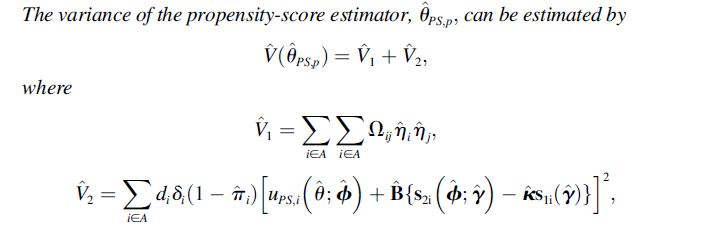
\includegraphics[width=1\linewidth]{var.jpg}
\end{figure}
\end{frame}

%------------------------------------------------
%------------------------------------------------
\section{Simulation Study}
%------------------------------------------------
\begin{frame}
\frametitle{Simulation Study}
\underline{Setup}
\begin{itemize}
\item \e{x \sim N(0, 0.5)} and \e{y=m(x)+e} with four different mean structures and three different error models:\medskip
\item \e{m_1(x)=-1+x},\\ \e{m_2(x)=-2+0.5\exp(0.5+x)},\\ \e{m_3(x)=-1+\sin(2x)},\\ \e{m_4(x)=-1+0.4x^3},\medskip
\item \e{e \sim N(0, 0.9)},\\ \e{e \sim N\bra{0, 0.49\bra{1+x^2}}},\\ \e{e \sim \ln N(-0.49/2, 0.49)}.\medskip
\end{itemize}
\end{frame}

\begin{frame}
\frametitle{Simulation Study}
\underline{Setup}
\begin{itemize}
\item \e{\delta_i \sim \text{ Ber}\bra{\pi_i}}\\where \e{\pi_i = \cbra{1+\exp\bra{-\phi_0-\phi_1y_i}}^{-1}}\\
		with \e{\bra{\phi_0, \phi_1}=(0.8, -0.2)}\medskip
\item estimate \e{\theta=E\bra{Y}} with the following five methods:\\
	 1. Full Sample (assume all data observed)\\
	 2. Missing At Random (ignorable nonresponse)\\
	 3. Fully Parametric (FP)\\
	 4. Generalized Method of Moments (GMM)\\
	 5. New Method
\end{itemize}
\end{frame}

\begin{frame}
\frametitle{Simulation Study}
\begin{figure}
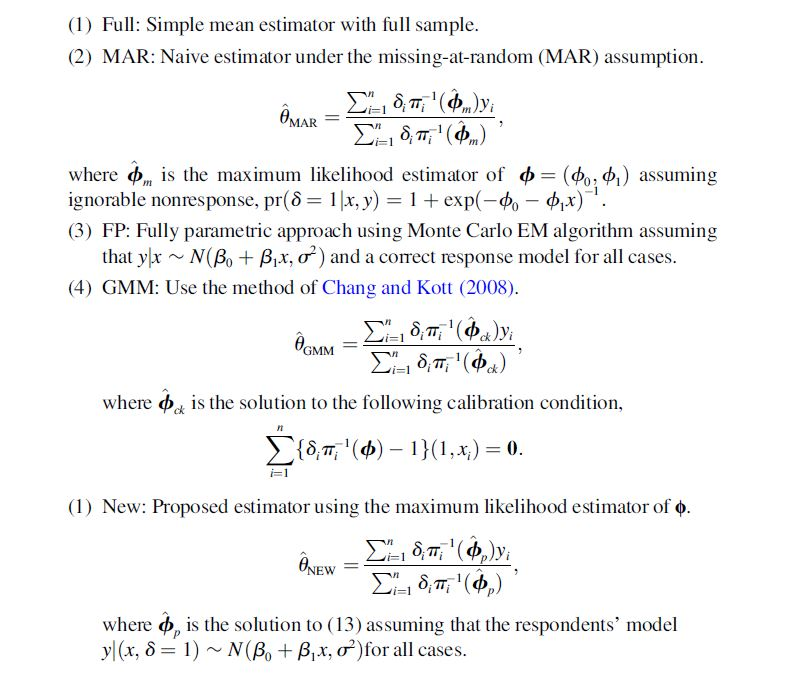
\includegraphics[width=0.7\linewidth]{solver.jpg}
\end{figure}
\end{frame}

\begin{frame}
\frametitle{Simulation Study}
\centerline{n = 500, B = 2000}
\begin{figure}
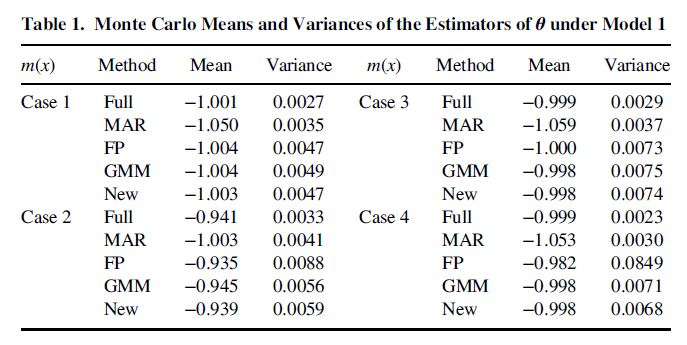
\includegraphics[width=1\linewidth]{table1.jpg}
\end{figure}
\end{frame}
\begin{frame}
\frametitle{Simulation Study}
\centerline{n = 500, B = 2000}
\begin{figure}
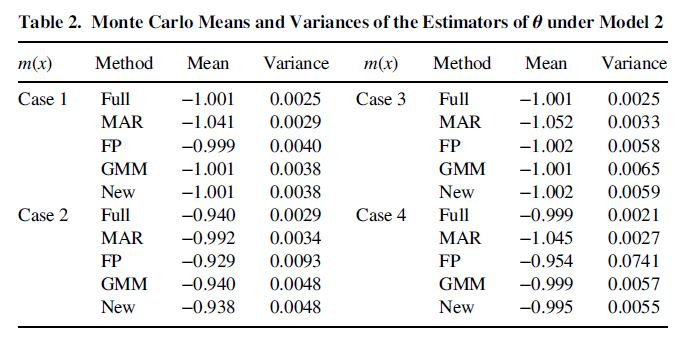
\includegraphics[width=1\linewidth]{table2.jpg}
\end{figure}
\end{frame}
\begin{frame}
\frametitle{Simulation Study}
\centerline{n = 500, B = 2000}
\begin{figure}
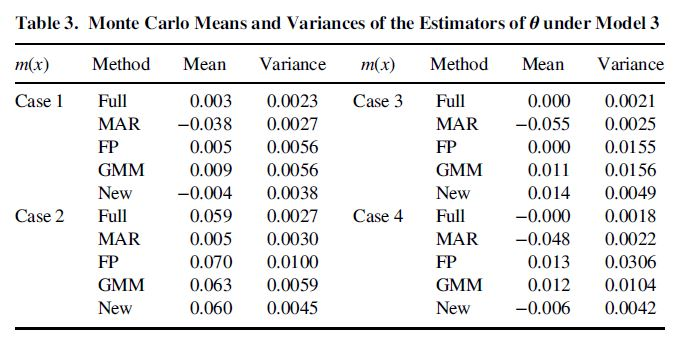
\includegraphics[width=1\linewidth]{table3.jpg}
\end{figure}
\end{frame}

\begin{frame}
\frametitle{Simulation Study}
\centerline{n = 200, B = 1000}
\begin{figure}
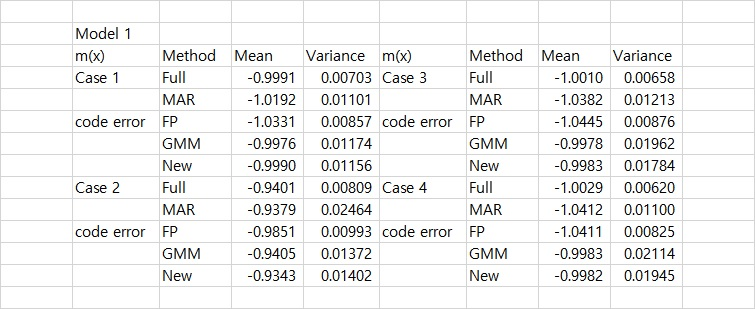
\includegraphics[width=1\linewidth]{res1.jpg}
\end{figure}
\end{frame}
\begin{frame}
\frametitle{Simulation Study}
\centerline{n = 200, B = 1000}
\begin{figure}
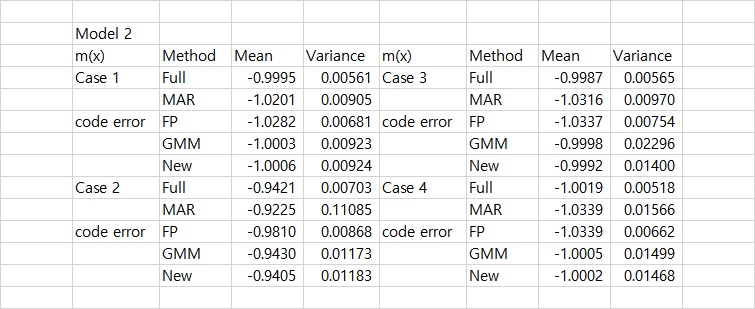
\includegraphics[width=1\linewidth]{res2.jpg}
\end{figure}
\end{frame}
\begin{frame}
\frametitle{Simulation Study}
\centerline{n = 200, B = 1000}
\begin{figure}
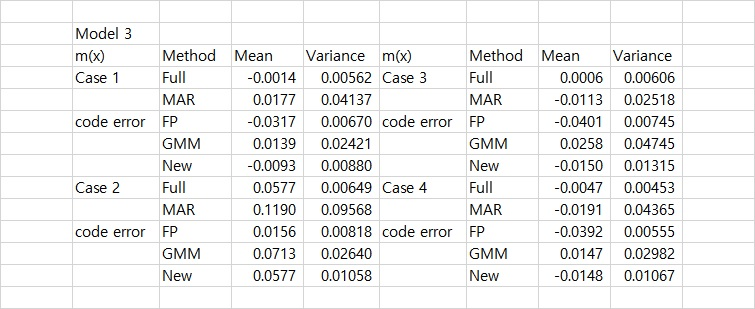
\includegraphics[width=1\linewidth]{res3.jpg}
\end{figure}
\end{frame}

\begin{frame}
\frametitle{Simulation Study}
\centerline{n = 500, B = 2000}
\begin{figure}
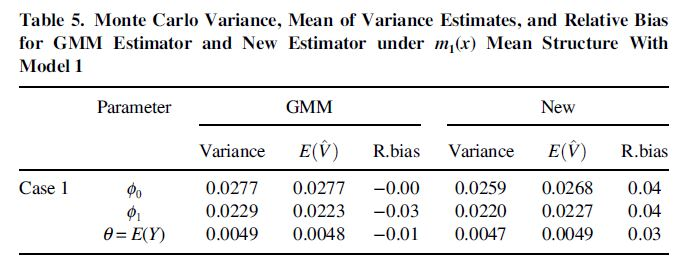
\includegraphics[width=1\linewidth]{table5.jpg}
\end{figure}
\end{frame}

%------------------------------------------------
%------------------------------------------------
\section{Conclusion and Remarks}
%------------------------------------------------

\begin{frame}
\frametitle{Conclusion and Remarks}
\begin{itemize}
\item New MLE method for nonignorable nonresponse.\smallskip
\item It is based on \e{f\bra{y|x,\delta=1}} and the result is not sensitive. In the simulation we use normal distribution for \e{f\bra{y|x,\delta=1}}, but the resulting estimates are nearly unbiased.\smallskip
\item It is efficient since it is based on MLE approach. However, it doesn't necessarily satisfy the calibration constraints, so there is still room for improvement.\smallskip
\item It provides consistent estimates for the standard errors. Thus, we can test the null hypothesis that the response mechanism is ignorable. So, we can do some pretest procedure, and furthre investigation on this direction will be a topic of future research.
\end{itemize}
\end{frame}

\begin{frame}
\centerline{\huge{Question?}}
\end{frame}

\end{document} 